%!TEX TS-program = xelatex
\documentclass[12pt,a4paper, oneside]{extreport}

%%%%%%%%%% Математика %%%%%%%%%%
\usepackage{amsmath,amsfonts,amssymb,amsthm,mathtools}
% Показывать номера только у тех формул, на которые есть \eqref{} в тексте.
%\mathtoolsset{showonlyrefs=true}
%\usepackage{leqno} % Нумерация формул слева
%\usepackage{tipa} %Для формулки из логитов


\usepackage{hyphenat}


%%%%%%%%%% Шрифты %%%%%%%%
\usepackage[english, russian]{babel} % выбор языка для документа
\usepackage[utf8]{inputenc} % задание utf8 кодировки исходного tex файла
\usepackage[X2,T2A]{fontenc}        % кодировка

\usepackage{fontspec}         % пакет для подгрузки шрифтов
\setmainfont{Times New Roman}       % задаёт основной шрифт документа

\usepackage{unicode-math}      % пакет для установки математического шрифта
\setmathfont{Asana-Math.otf}    % шрифт для математики

% Конкретный символ из конкретного шрифта
% \setmathfont[range=\int]{Neo Euler}




%%%%%%%%%% Работа с картинками %%%%%%%%%
\usepackage{graphicx}                  % Для вставки рисунков
\usepackage{graphics}
\graphicspath{{images/}{pictures/}}    % можно указать папки с картинками
\usepackage{wrapfig}                   % Обтекание рисунков и таблиц текстом


%%%%%%%%%% Работа с таблицами %%%%%%%%%%
\usepackage{tabularx}            % новые типы колонок
\usepackage{tabulary}            % и ещё новые типы колонок
\usepackage{array,delarray}      % Дополнительная работа с таблицами
\usepackage{longtable}           % Длинные таблицы
\usepackage{multirow}            % Слияние строк в таблице
\usepackage{float}               % возможность позиционировать объекты в нужном месте

\usepackage{booktabs}            % таблицы как в книгах
% Заповеди из документации к booktabs:
% 1. Будь проще! Глазам должно быть комфортно
% 2. Не используйте вертикальные линни
% 3. Не используйте двойные линии. Как правило, достаточно трёх горизонтальных линий
% 4. Единицы измерения - в шапку таблицы
% 5. Не сокращайте .1 вместо 0.1
% 6. Повторяющееся значение повторяйте, а не говорите "то же"
% 7. Есть сомнения? Выравнивай по левому краю!

%  вычисляемые колонки по tabularx
\newcolumntype{C}{>{\centering\arraybackslash}X}
\newcolumntype{L}{>{\raggedright\arraybackslash}X}
\newcolumntype{Y}{>{\arraybackslash}X}
\newcolumntype{Z}{>{\centering\arraybackslash}X}


%%%%%%%%%% Графика и рисование %%%%%%%%%%
\usepackage{tikz, pgfplots}      % язык для рисования графики из latex'a

%%%%%%%%%% Гиперссылки %%%%%%%%%%
\usepackage{xcolor}              % разные цвета

\usepackage{hyperref}
\hypersetup{
	unicode=true,           % позволяет использовать юникодные символы
	colorlinks=true,       	% true - цветные ссылки, false - ссылки в рамках
	urlcolor =blue,         % цвет ссылки на url
	linkcolor=black,        % внутренние ссылки
	citecolor=black,        % на библиографию
	breaklinks              % если ссылка не умещается в одну строку, разбивать ли ее на две части?
}


%%%%%%%%%% Другие приятные пакеты %%%%%%%%%
\usepackage{multicol}       % несколько колонок
\usepackage{verbatim}       % для многострочных комментариев
\usepackage{cmap} % для кодировки шрифтов в pdf

\usepackage{enumitem} % дополнительные плюшки для списков
%  например \begin{enumerate}[resume] позволяет продолжить нумерацию в новом списке

\usepackage{todonotes} % для вставки в документ заметок о том, что  осталось сделать
% \todo{Здесь надо коэффициенты исправить}
% \missingfigure{Здесь будет Последний день Помпеи}
% \listoftodos --- печатает все поставленные \todo'шки



%%%%%%%%%%%%%% ГОСТОВСКИЕ ПРИБАМБАСЫ %%%%%%%%%%%%%%%

%%% размер листа бумаги
\usepackage[paper=a4paper,top=15mm, bottom=15mm,left=35mm,right=10mm,includehead]{geometry}


\usepackage{setspace}
\setstretch{1.33}     % Межстрочный интервал
\setlength{\parindent}{1.5em} % Красная строка.


%\flushbottom       % Эта команда заставляет LaTeX чуть растягивать строки, чтобы получить идеально прямоугольную страницу
\righthyphenmin=2  % Разрешение переноса двух и более символов
\widowpenalty=10000  % Наказание за вдовствующую строку (одна строка абзаца на этой странице, остальное --- на следующей)
%\clubpenalty=10000  % Наказание за сиротствующую строку (омерзительно висящая одинокая строка в начале страницы)
\tolerance=1000     % Ещё какое-то наказание.


% Нумерация страниц сверху по центру
\usepackage{fancyhdr}
\pagestyle{fancy}
\fancyhead{ } % clear all fields
\fancyfoot{ } % clear all fields
\fancyhead[C]{\thepage}
% Чтобы не прорисовывалась черта!
\renewcommand{\headrulewidth}{0pt}


% Нумерация страниц с надписью "Глава"
\usepackage{etoolbox}
\patchcmd{\chapter}{\thispagestyle{plain}}{\thispagestyle{fancy}}{}{}


%%% Заголовки
\usepackage[indentfirst]{titlesec}{\raggedleft}
% Заголовки по левому краю
% опция identfirst устанавливает отступ в первом абзаце



% В Linux этот пакет сделан косячно. Исправляет это следующий непонятный кусок кода.
\makeatletter
\patchcmd{\ttlh@hang}{\parindent\z@}{\parindent\z@\leavevmode}{}{}
\patchcmd{\ttlh@hang}{\noindent}{}{}{}
\makeatother


% Редактирования Глав и названий
\titleformat{\chapter}
{\normalfont\large\bfseries}
{\thechapter }{0.5 em}{}

% Редактирование ненумеруемых глав chapter* (Введение и тп)
\titleformat{name=\chapter,numberless}
{\centering\normalfont\bfseries\large}{}{0.25em}{\normalfont}

% Убирает чеканутые отступы вверху страницы
\titlespacing{\chapter}{0pt}{-\baselineskip}{\baselineskip}

% Более низкие уровни
\titleformat{\section}{\bfseries}{\thesection}{0.5 em}{}
\titleformat{\subsection}{\bfseries}{\thesubsection}{0.5 em}{}

\titlespacing*{\section}{0 pt}{\baselineskip}{\baselineskip}
\titlespacing*{\subsection}{0 pt}{\baselineskip}{\baselineskip}


% Содержание. Команды ниже изменяют отступы и рисуют точечки!
\usepackage{titletoc}

\titlecontents{chapter}
[1em] %
{\normalsize}
{\contentslabel{1 em}}
{\hspace{-1 em}}
{\normalsize\titlerule*[10pt]{.}\contentspage}

\titlecontents{section}
[3 em] %
{\normalsize}
{\contentslabel{1.75 em}}
{\hspace{-1.75 em}}
{\normalsize\titlerule*[10pt]{.}\contentspage}

\titlecontents{subsection}
[6 em] %
{\normalsize}
{\contentslabel{3 em}}
{\hspace{-3 em}}
{\normalsize\titlerule*[10pt]{.}\contentspage}


% Правильные подписи под таблицей и рисунком
% Документация к пакету на русском языке!
\usepackage[tableposition=top, singlelinecheck=false]{caption}
\usepackage{subcaption}


\DeclareCaptionStyle{base}%
[justification=centering,indention=0pt]{}
\DeclareCaptionLabelFormat{gostfigure}{Рисунок #2}
\DeclareCaptionLabelFormat{gosttable}{Таблица #2}

\DeclareCaptionLabelSeparator{gost}{~---~}
\captionsetup{labelsep=gost}

\DeclareCaptionStyle{fig01}%
[margin=5mm,justification=centering]%
{margin={3em,3em}}
\captionsetup*[figure]{style=fig01,labelsep=gost,labelformat=gostfigure,format=hang}

\DeclareCaptionStyle{tab01}%
[margin=5mm,justification=centering]%
{margin={3em,3em}}
\captionsetup*[table]{style=tab01,labelsep=gost,labelformat=gosttable,format=hang}


% межстрочный отступ в таблице
\renewcommand{\arraystretch}{1.2}



% многостраничные таблицы под РОССИЙСКИЙ СТАНДАРТ
% ВНИМАНИЕ! Обязательно за CAPTION !
\usepackage{fr-longtable}



%Более гибкие спсики
\usepackage{enumitem}
% сообщаем окружению о том, что существует такая штук как нумерация русскими буквами.
\makeatletter
\AddEnumerateCounter{\asbuk}{\russian@alph}{щ}
\makeatother


%%% ГОСТОВСКИЕ СПИСКИ

% Первый тип списков. Большая буква.
\newlist{Enumerate}{enumerate}{1}

\setlist[Enumerate,1]{labelsep=0.5em,leftmargin=1.25em,labelwidth=1.25em,
	parsep=0em,itemsep=0em,topsep=0ex, before={\parskip=-1em},label=\arabic{Enumeratei}.}


% Второй тип списков. Маленькая буква.
\setlist[enumerate]{label=\arabic{enumi}),parsep=0em,itemsep=0em,topsep=0.75ex, before={\parskip=-1em}}


% Третий тип списков. Два уровня.
\newlist{twoenumerate}{enumerate}{2}
\setlist[twoenumerate,1]{itemsep=0mm,parsep=0em,topsep=0.75ex,, before={\parskip=-1em},label=\asbuk{twoenumeratei})}
\setlist[twoenumerate,2]{leftmargin=1.3em,itemsep=0mm,parsep=0em,topsep=0ex, before={\parskip=-1em},label=\arabic{twoenumerateii})}


% Четвёртый тип списков. Список с тире.
\setlist[itemize]{label=--,parsep=0em,itemsep=0em,topsep=0ex, before={\parskip=-1em},after={\parskip=-1em}}


%%% WARNING WARNING WARNIN!
%%% Если в списке предложения, то должна по госту стоять точка после цифры => команда Enumerate! Если идет перечень маленьких фактов, не обособляемых предложений то после цифры идет скобка ")" => команда enumerate! Если перечень при этом ещё и двууровневый, то twoenumerate.




%%%%%%%%%% Список литературы %%%%%%%%%%

%\usepackage[%
%backend=biber, %подключение пакета biber (тоже нужен)
%bibstyle=gost-numeric, %подключение одного из четырех главных стилей biblatex-gost
%sorting=ntvy, %тип сортировки в библиографии
%]{biblatex}
\usepackage[backend=biber,style=gost-numeric, maxbibnames=9,maxcitenames=2,uniquelist=false, babel=other]{biblatex}

% Справка по 4 главным стилям для ленивых:
% gost-inline  ссылки внутри теста в круглых скобках
% gost-footnote подстрочные ссылки
% gost-numeric затекстовые ссылки
% gost-authoryear тоже затекстовые ссылки, но немного другие

% Подробнее смотри страницу 4 документации. Она на русском.

% Ещё немного настроек
\DeclareFieldFormat{postnote}{#1} %убирает с. и p.
\renewcommand*{\mkgostheading}[1]{#1} % только лишь убираем курсив с авторов


\addbibresource{diplomabib.bib} % сюда нужно вписать свой bib-файлик.

% Этот кусок кода выносит русские источники на первое место. Костыль описали авторы пакета в руководстве к нему. Подробнее смотри:
% https://github.com/odomanov/biblatex-gost/wiki/Как-сделать%2C-чтобы-русскоязычные-источники-предшествовали-остальным
\DeclareSourcemap{
	\maps[datatype=bibtex]{
		\map{
			\step[fieldsource=langid, match=russian, final]
			\step[fieldset=presort, fieldvalue={a}]
		}
		\map{
			\step[fieldsource=langid, notmatch=russian, final]
			\step[fieldset=presort, fieldvalue={z}]
		}
	}
}

\DefineBibliographyStrings{english}{%
	pages = {P\adddot},
	number = {№},
}


\begin{document} % Начала документа

\thispagestyle{empty} % Чтобы избежать нумерации титульника

% Если для какой-то страницы хочется сделать своё уникальное оформление, как например для титульника или списка литературы, то можно использовать окружение \begingroup ... \endgroup. 
\begingroup
\setstretch{1}   % Убираем полторашные интервалы на титульнике
\begin{center}
\small \bfseries Федеральное государственное бюджетное образовательное учреждение высшего образования

<<РОССИЙСКАЯ АКАДЕМИЯ НАРОДНОГО ХОЗЯЙСТВА и\\ ГОСУДАРСТВЕННОЙ СЛУЖБЫ \\
при Президенте Российской Федерации>>

\vspace{2ex}

\bfseries
ИНСТИТУТ ЭКОНОМИКИ, МАТЕМАТИКИ И ИНФОРМАЦИОННЫХ 

ТЕХНОЛОГИЙ
 
 ЭКОНОМИЧЕСКИЙ ФАКУЛЬТЕТ 
 
НАПРАВЛЕНИЕ 38.03.01 ЭКОНОМИКА

\end{center}

\vfill


\noindent  Группа ЭО-15-01
\hfill
\parbox[t]{20em}{\centering
Кафедра микроэкономики

\mbox{ }

\textbf{Допустить к защите}

заведующий кафедрой микроэкономики

\mbox{ }

\rule{8em}{0.5pt} М.И. Левин

\mbox{ }

<<\rule{2em}{0.5pt}>> \rule{5em}{0.5pt} 201\rule{1em}{0.5pt} г. }

\mbox{ }

\mbox{ }

\begin{center}\bfseries
ВЫПУСКНАЯ КВАЛИФИКАЦИОННАЯ РАБОТА

\mbox{ }

\large
ПРОГНОЗИРОВАНИЕ   \\
ИЕРАРХИЧЕСКИХ ВРЕМЕННЫХ РЯДОВ
\end{center}

\vfill

\noindent\normalsize
студент-бакалавр

\noindent
Касьянова Ксения Алексеевна
\hfill /\rule{6em}{0.5pt}/\rule{6em}{0.5pt}/

\hfill\makebox[13em]{\hfill\footnotesize (подпись) \hfill\hfill (дата) \hfill}

\noindent
научный руководитель выпускной \\
квалификационной работы

\noindent
ст. преп. Демешев Борис Борисович
\hfill /\rule{6em}{0.5pt}/\rule{6em}{0.5pt}/

\hfill\makebox[13em]{\hfill\footnotesize (подпись) \hfill\hfill (дата) \hfill}

%\noindent
%консультант
%
%\noindent
%д.э.н., профессор Петров Петр Петрович
%\hfill /\rule{6em}{0.5pt}/\rule{6em}{0.5pt}/
%
%\hfill\makebox[13em]{\hfill\footnotesize (подпись) \hfill\hfill (дата) \hfill}

\vfill

\begin{center}
\normalsize \bfseries МОСКВА \\ 2019 г.
\end{center}
\endgroup



%%%%%%%%%%%%%%%%%%% ОГЛАВЛЕНИЕ %%%%%%%%%%%%%%%%%%%%%%%%%%%%%%%%%%%%%%

\tableofcontents  % Команда, которая создаёт оглавление


%%%%%%% ВВЕДЕНИЕ %%%%%%

\chapter*{Введение}
%Включение введения в соодержание
\addcontentsline{toc}{chapter}{Введение}


В анализе данных часто встречаются данные со сложной многоуровневой структурой, точный прогноз которых является одним из ключевых факторов принятия эффективных решений. В связи с этим необходимо использовать уже известные подходы, позволяющие учитывать взаимозависимости прогнозируемых временных рядов, и разрабатывать новые.  


С развитием различных социально-экономических процессов, укрепляется и взаимосвязь между ними. Анализ данных с иерархической структурой требуется в микроэкономике (например, при анализе спроса на различные виды товаров в разных городах), макроэкономике (показатели выпуска по регионам по разным отраслям), страховании (анализ рисков попасть аварию, в зависимости от привычек и местонахождения человека),  демографии (смертность по регионам и причинам смерти) и т.д.  Помимо этого существует и межвременная агрегация временных рядов, часто применяющаяся при прогнозировании.  

В данной работе исследуются методы прогнозирования иерархических временных рядов, учитывающие зависимость между уровнями агрегирования и внутри одного уровня. Теоретической основой исследования послужили работы ученых в области анализа данных, прогнозирования и моделирования.



Цель работы: сравнение моделей, учитывающих иерархическую структуру данных, выявление факторов, позволяющих улучшить прогнозы агрегированного временного ряда.

%используя модели, учитывающие иерархическую структуру данных, улучшить прогнозы агрегированного временного ряда.

%использовать информацию на одном уровне агрегирования для улучшения прогнозов на другом уровне агрегирования. 

Достижение поставленной цели предполагает постановку и решение следующих задач:

\begin{itemize}
	\item сбор данных с трехуровневой иерархической структурой;
	\item выбор моделей для прогнозирования агрегированного ряда;
	\item сравнение ARIMA моделей с использованием дополнительных регрессоров (ближайшего по метрике корреляции временного ряда третьего уровня, ряда второго уровня или прогноза ряда второго уровня) и без;    
	\item сравнение различных методов комбинирования прогнозов нижних рядов; 
	\item кластеризация временных рядов третьего уровня для получения комбинированных рядов второго уровня (суммирование всех рядов, попавших в один кластер), сравнение прогнозов по  "оригинальным" и "комбинированным" рядам второго уровня;
	\item прогнозирование рядов второго и третьего уровня по выбранным моделям, сравнение суммы и оптимальной комбинации этих прогнозов с прогнозом агрегированного временного ряда.
%	\item сравнение прогнозной силы моделей для агрегированного временного ряда, взвешенных прогнозов дизагрегированных рядов; % и иерархической байесовской модели.
%\item  Добавление в модель дамми структурного сдвига

\end{itemize}


%Актуальность
Методы, описанные в данной работе актуальны при необходимости прогнозирования, как агрегированного ряда, так и отдельных компонент, составляющих его, а также получения подтверждения правильности выбора модели для агрегированного ряда.
Для анализа были выбраны ряды с определенной структурой, а именно: 
структура трехуровневая и иерархическая, причем сам агрегированный ряд и ряды второго уровня можно получить при суммировании рядов третьего уровня. 
%В ходе исследования мы определим,  позволяет ли такое детальное дробление временного ряда на более мелкие добиться существенного улучшения прогнозов или можно, например, ограничиться двумя уровнями.


% теоретическую и практическую значимость работы (если работа претендует на значи-мые результаты в этих аспектах)

Практическая значимость работы заключается в том, что при анализе результатов применения изучаемых методов на трех наборах данных (с разной сезонностью, числом наблюдений и рядов на каждом уровне)   с использованием перекрестной проверки (кросс-валидации) можно протестировать методы на независимых данных, а следовательно получить более устойчивые  выводы. 



Данная работа состоит из введения, двух глав основной части, заключения и приложений. В первой главе рассматриваются основные модели прогнозирования иерархических временных рядов.  Во второй главе проводится  сравнение моделей применительно к собранным данным с требуемой структурой. 

%В данной работе мной был проведен анализ моделей роста (Приложение А), на основе
%которого была выбрана модель, наилучшим образом описывающая потребление ограничен-
%ного ресурса. В дополнение результатов, уже полученных авторами модели, мною были под-
%тверждены и прокомментированы некоторые условия (пункт 2.3), которые у авторов работы
%шли без доказательства. Самый главный вывод, сделанный мной, был получен в ходе анали-
%за данной модели в отношении динамики запаса ресурса. На эти детали авторы работы свое
%внимание не обратили, но я считаю, что он как раз показывает всю важность применения
%методов стохастического анализа при моделировании запасов ограниченного ресурса. Эти
%выводы представлены в пункте 2.5., а также визуализированы мной с помощью MATLAB
%(пункт 3.2)


% степень ее разработанности


%методологию и методы исследования;

%положения, выносимые на защиту;



\chapter{Модели прогнозирования временных рядов с иерархической структурой}



\section{Обзор литературы}

Одним из способов повышения точности прогнозов является агрегирование данных. Один из вариантов - агрегирование временных рядов до составления прогноза, другой - агрегирование самих прогнозов. 

С другой стороны информация полученная из аггрегированных рядов может иметь существенное влияние при прогнозировании рядов нижнего уровня, хотя ее использование может сопровождаться некоторыми сложностями. 

Для наиболее распространенных моделей прогнозированию существуют альтернативные подходы к анализу временных рядов с иерархической структурой, например, модель  векторной авторегрессии (VAR), в которой  временные ряды имеют общие параметры или модель байесовской векторной авторегрессии (BVAR), где коэффициенты  при различных регрессорах могут иметь общее априорное распределение.  В том числе применяются многомерные модели пространства состояний, векторное  экспоненциальное сглаживание, а также  байесовские подходы, например, их применение к пулу аналогичных временных рядов с помощью ... [Duncan et al. (1993, 2001)].
В таких моделях обычная оценка параметрами объединяется с оцененкой по сгруппированной модели. 

Эмпирические результаты показали, что с помощью перечисленных выше методов точность прогноза может быть улучшена, поскольку они используют ковариационную зависимость  между временными рядами. Однако использование их связано с выполнением большого числа предпосылок или введения соответствующих ограничений на модель.


Эти методы по крайней мере теоретически могут легко обогнать по качеству прогнозов такие простые подходы, как bottom-up (BU), top-down (TD).
Но помимо BU и TD подходов к получению прогнозов аггрегированных рядов, существуют более сложные методы получения  оптимальных комбинаций прогонозов, например, ...
Однако во многих теоретических и эмпирических работах было замечено, что зачастую более простые методы комбинирования прогнозов оказываются в разы эффективнее, сложных методов, использующих метррики, учитывающие особенности каждого из рядов. Так, например, в статье ... лучший прогноз давало простое взвешивание прогнозов. 



\section{Использование дополнительных регрессоров в ARIMA моделях}

Одной из наиболее распространенных моделей прогнозирования взаимозависимых рядов является модель векторной авторегрессии (VAR), однако ее использование может сопровождаться некоторыми сложностями, большое число лагов в модели приводит к громоздким методам вычисления оценок коэффициентов.  

В качестве некой альтернативы этому методу можно предложить использование модели ARIMA с дополнительными регрессорами, полученными из прогнозируемого набора данных. 




\section{Взвешенные прогнозы}

Тем не менее менее существует мнение, что оптимальным уровнем прозрачности работы центрального банка является некоторый промежуточный уровень. Как это ни парадоксально, высокий уровень прозрачности деятельности ЦБ может привести к неопределенности.  Слишком большой объем информации приводит к перегрузке и путанице%~\cite{morris2005central}.

% Обратите внимание на непрерывный пробел около сноски! Это делается для того, чтобы сноска не улетела от предложения на отдельную строку. И не возникло уродливой цифры в отдельной строке.

\section{Иерархический Байес}

%    - HB (Иерархический Байес с выделением разных групп  по разным метрикам кластеризации)



\chapter{Сравнение моделей прогнозирования}





\section{Описание данных}

Для анализа  необходимо найти наборы данных удовлетворяющие следующим критериям: 
структура трехуровневая и иерархическая, обладающая свойством аддитивности, т.е. для $I$ рядов второго уровня, каждый из которых делится на $J$ рядов третьего уровня, выполняется: 

\begin{equation}\label{key}
y_t = \sum_{i=1}^I y_{i,t} = \sum_{i=1}^I \sum_{j=1}^J y_{ij,t} 
\end{equation}

где $y_{ij,t}, y_{i,t},  y_{t}  $ - значения $j$-ого ряда третьего уровня, $i$-ого ряда второго уровня и ряда первого уровня соответственно в момент времени $t$. 


Стоит отметить, что поиск реальных данных, идеально подходящих под такую структуру, затруднен. Обычно для микроэкономических показателей  в первую очередь собираются данные по отдельным компонентам, из которых  можно получить агрегированные ряды, что удовлетворяет свойству аддитивности, однако получить доступ к таким данным сложно. Альтернативой являются макроэкономические данные, при использовании которых стоит учесть, что в общем случае значение верхнего ряда не будет в точности  равно сумме нижних рядов, по причине различий в методологиях сбора рядов разных уровней используемых для   избежания двойного учета, неточностей и прочих проблем. 

Так например, разбивая ряд ВВП на компоненты по регионам и отраслям, надо учесть, что вообще компоненты будут отражать несколько иной показатель -  валовую добавленную стоимостью (ВДС)~\footnote{Валовая добавленная стоимость определяется как разность между выпуском товаров и услуг и их промежуточным потреблением. ВДС  исчисляется на уровне отраслей и отражает образование первичных доходов в результате процесса производства товаров и услуг.}. Агрегированный ряд, получаемый при суммировании всех ВДС, будет меньше ВВП на величину чистых субсидий на производство и импорт. Такой показатель имеет близкую к единице корреляцию с рядом ВВП, поэтому при точном его прогнозировании мы можем получить представление как об общей динамике всех компонент, составляющих ряд, так и о динамике ряда ВВП.  Поскольку целью работы является сравнение моделей, для упрощения будем работать с агрегированными показателями по ВВП, являющиеся простой суммой из рядов нижнего уровня. 


Вообще говоря, этот  факт учитывается при расчете вклада компонент, составляющих ряд, в процентное изменение агрегированного показателя, не обладающего свойством аддитивности~\footfullcite{bea3}:  

\begin{equation}\label{key}
 C\% Δ_{i,t} = 100 * \dfrac{q_{i,t}-q_{i,t-1} }{\sum_j q_{j,t-1} } 
\end{equation}

где $q_{i,t}$ - значение $i$-ого ряда в момент времени $t$.

Такой показатель позволяет определить изменения в структуре агрегата, что делает его ценным инструментом экономического анализа.
Если при прогнозировании с помощью иерархических моделей удастся улучшить прогноз агрегированного ряда, то фактически мы также сможем получить достаточно точные прогнозы показателей вклада каждой компоненты.

Для анализа были выбраны три набора данных с описанными выше свойствами, обладающие  разной сезонностью:  квартальные, квартальные сезонно сглаженные и месячные данные.  


\subsection{Квартальные данные}

Квартальные данные\footfullcite{eurostat1} - ряды ВДС по 28 странам Европейского союза (включая Великобританию) в разбивке по основным отраслям\footfullcite{eurostat2}:

\begin{enumerate}
	\item  'A' - сельское хозяйство, лесное хозяйство и рыболовство;
\item  'B' - промышленность (кроме строительства);
\item  'F' - строительство;
\item  'G'- оптовая и розничная торговля, транспорт, услуги общественного питания и т.д.;
\item  'J'- информация и связь;
\item  'K'- финансовая и страховая деятельность;
\item  'L'- операции с недвижимостью;
\item  'M'- профессиональная, научно-техническая, административная деятельность;
\item  'O'- государственное управление, оборона, образование, здравоохранение и социальная работа;
\item  'R'- искусство, развлечения, отдых и другие виды услуг. 

Данные собраны за период с 2000-Q1 по 2018-Q3. 


\end{enumerate}

%\begin{figure}
%	\centering
%	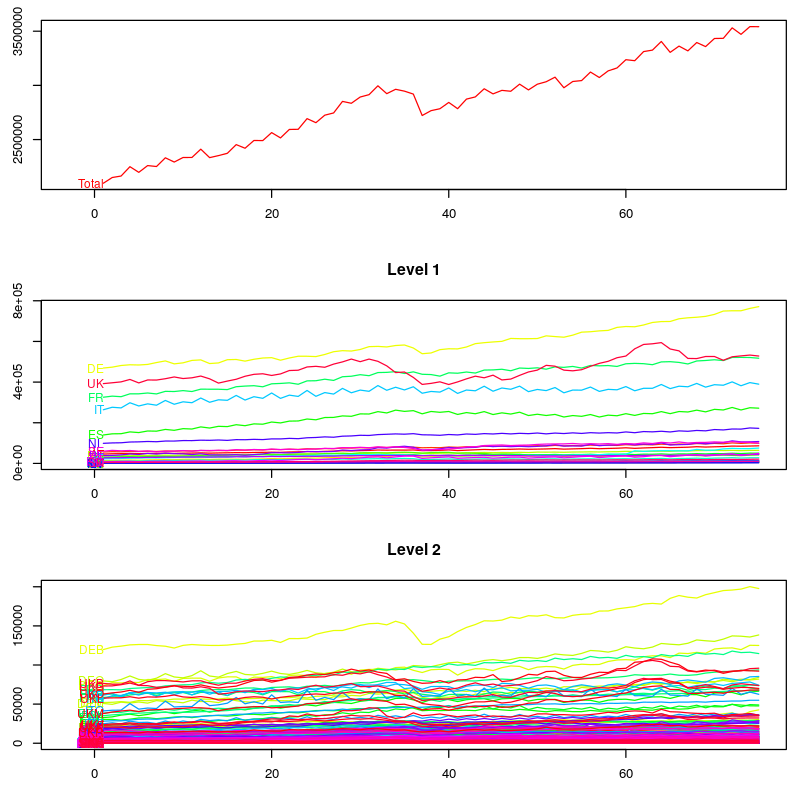
\includegraphics[width=0.7\linewidth]{screenshot001}
%	\caption[Квартальные временные ряды]{Квартальные временные ряды}
%	\label{fig:screenshot001}
%\end{figure}

Разница между совокупным ВВП всех 28 стран, входящих в состав ЕС  и суммой ВДС по всем отраслям для каждого из государств, не превышает  1.5\% от ВВП. 

\subsection{Квартальные сезонно сглаженные данные}

Квартальные сезонно сглаженные данные~\footfullcite{usstat1} - это ряды ВДС  для каждого из 50 штатов Америки с разбивкой на 21 отрасль.  Данные собраны за период с 2005-Q1 по 2018-Q2. 


В этом наборе 11 рядов имели пропуски. По четырем из них  данные перестали собираться в 2008 году, поэтому эти ряды были исключены целиком. Остальные пропуски  были заполнены с помощью экспоненциально взвешенного скользящего среднего с шириной окна 4~\footnote{Алгоритм, используемый в пакете R "imputeTS" имеет адаптивный размер окна: в случае длинных промежутков с пропущенными значениями, размер окна постепенно увеличивается до тех пор, пока не появятся как минимум 2 значения не-NA. }. 

Квартальные оценки ВДС в США пересчитываются с учетом сезонных колебаний следующим образом: BEA оценивает соответствующие коэффициенты сезонной корректировки, после чего удаляет из временного ряда среднее влияние изменений, которые обычно происходят примерно в одно и то же время  с одинаковой величиной каждый год. Сезонно несглаженные ряды по этому показателю BEA не публикует.

Показатели по ВДС публикуются в реальном денежном эквиваленте (за базовый год принимается 2012).
Надо отметить, что  значения реальных показателей ВДС по отраслям не обязательно дают в сумме показатель реального ВДС для каждого штата за интересующий период, поскольку относительные цены, используемые в качестве весов для корректировки показателей по отраслям, отличаются от общего уровня цен используемых для корректировки агрегированного показателя. 
Для периодов близких к 2012 году, когда значительных отклонений относительных цен от индекса цен по стране не было, показатель ВДС штата совпадает с суммой ВДС по отраслям, хотя  вообще эта разница не превышает 0.5\% ВВП.
Разница между ВВП США и суммой ВДС по отраслям для каждого штата не превышает 2\%. 


\subsection{Месячные данные}

Месячные данные\footfullcite{fedstat1} - показатели рождаемости и смертности по основным причинам  в каждом регионе РФ, дающие в сумме естественный прирост населения помесячно. 
Данные собраны за период с 2006-01 по 2019-01. 


Если для каждого из регионов просуммировать по причинам смерти все показатели из набора данных "Число зарегистрированных умерших по основным классам и отдельным причинам смерти (оперативные данные)", значения будут отличаться от показателей набора данных "Число зарегистрированных умерших (оперативные данные)". Такое расхождение объясняется тем, что по первому показателю  разрабатываются не все причины смерти, а только основные классы и отдельные причины смерти, имеющие наибольший вес. Также в 2011 году методика разработки показателя была пересмотрена, чтобы соответствовать  Международной статистической классификации\footfullcite{fedstat2}. 

В связи с этим для анализа были выявлены три основные группы причин смертности, причем разница между показателем смертности по каждому региону и суммой по всем причинам смертности была добавлена к ряду "смерть по прочим причинам":  



\begin{enumerate}
	\item  'УБ' - смерть из-за болезней (болезней органов дыхания, органов пищеварения, системы кровообращения, инфекционных и паразитарных болезней, новообразований);
\item 'УУ'  -  убийство и самоубийство;
\item 'УВ'  -  смерть по прочим причинам (отравление алкоголем, транспортные травмы всех видов и внешние причины)
\end{enumerate}


С 2015 года также собираются данные по республике Крым и городу федерального значения Севастополю. Однако данных нужной сезонности и классификации за 2006-2014 годы Держстат Украины не предоставляет, поэтому ряды по этим регионам были исключены из набора данных. 



%- http://www.ukrcensus.gov.ua Держастат Украины

\section{Описание моделей прогнозирования рядов }

\subsection*{Сравнение качества прогнозов}

Для сравнения качества прогнозов будут использоваться следующие метрики:
\begin{itemize}
	\item  Средняя ошибка (mean error)
\begin{equation}\label{key}
ME = \frac{1}{h} \sum_{i=1}^h(\hat{y}_{t+i|t}-y_{t+i}) 
\end{equation}
\item  Квадратный корень из среднеквадратичной ошибки (root mean square error)
\begin{equation}\label{key}
RMSE = \sqrt{  \frac{1}{h} \sum_{i=1}^h(\hat{y}_{t+i|t}-y_{t+i})^2} 
\end{equation}
\item  Cредняя абсолютная ошибка в процентах  (mean absolute percentage error)
\begin{equation}\label{key}
MAPE = \frac{1}{h} \sum_{i=1}^h \frac{y_{t+i} - \hat{y}_{t+i|t} }{y_{t+i}} * 100\%
\end{equation}

\end{itemize}
Для выбора параметров модели будем сравнивать точность прогнозов по RMSE. Средняя ошибка позволит понять, насколько хорошо модель улавливает тренд в рядах. MAPE в качестве метрики сравнения точности прогнозов является смешенным показателем, поскольку он будет систематически выбирать модель, прогнозы которой занижены, так как MAPE налагает большие штрафы на отрицательные ошибки, чем на положительные. 
С расчетом MAPE для набора данных по России возникают трудности, так как в нем имеются нулевые и близкие к нулю значения.

\subsection{Кросс-валидация}

[Evaluating forecast accuracy](https://otexts.com/fpp2/accuracy.html)

\subsection{Кластеризация}

\subsection{Добавление регрессора}

\section{Сравнение моделей}



Функции импульсного отклика валютного курса, индекса РТС и ставки МИАКР на заявление Банка России при такой спецификации и идентифицирующих предположениях будут иметь вид, представленный на рис.%~\ref{otkl_1}. Функции импульсного отклика представлены с 95\% доверительными интервалами, построенными с помощью бутстрапа.

%\begin{figure}[h]
%\begin{minipage}[H]{0.49\linewidth}
%\center{\footnotesize{Валютный курс} \\\includegraphics[width=1\linewidth]{Rplot_USD}}
%\end{minipage}
%\hfill
%\begin{minipage}[H]{0.49\linewidth}
%\center{\footnotesize{Индекс РТС} \\ \includegraphics[width=1\linewidth]{Rplot_RTS}}
%\end{minipage}
%\vfill
%\begin{minipage}[H]{0.49\linewidth}
%\center{\footnotesize{Однодневная ставка МИАКР} \\\includegraphics[width=1\linewidth]{Rplot_MIACR}}
%\end{minipage}
%\caption{Функции импульсного отклика валютного курса, индекса РТС и ставки МИАКР на заявления Банка России}
%\label{otkl_1}
%\end{figure}

При словесной интервенции Банка России происходит прыжок однодневной ставки МИАКР в течение следующего дня после заявления. В течение четырёх дней ставка МИАКР возвращается к своему прежнему уровню. Вторая спецификация подтверждает выводы, полученные при первой спецификации модели. Импульсные отклики валютного курса и индекса РТС на словесные интервенции Банка России оказываются снова незначимыми.


\begin{table}[ht]
	\centering
	\begin{tabular}{rrrrr}
		\hline
		& ME & RMSE & MAPE & MASE \\ 
		\hline
		RW with drift  & 0.02 & 34.78 & 0.82 & 0.29 \\ 
		Auto ARIMA & 70.50 & 71.55 & 2.03 & 0.73 \\ 
		ARIMA & 72.67 & 73.73 & 2.09 & 0.75 \\ 
		RW & 77.53 & 100.92 & 2.52 & 0.91 \\ 
		ETS & 100.50 & 108.39 & 2.87 & 1.04 \\ 
		Theta & 103.38 & 109.50 & 2.96 & 1.07 \\ 
		SNaive & 134.86 & 146.04 & 3.86 & 1.40 \\ 
		\hline
	\end{tabular}
\end{table}

\begin{tabular}{rrrrr}
	\hline
	& ME & RMSE & MAPE & MASE \\ 
	\hline
	RW with drift  & 0.02 & 34.78 & 0.82 & 0.29 \\ 
	Auto ARIMA & 70.50 & 71.55 & 2.03 & 0.73 \\ 
	ARIMA & 72.67 & 73.73 & 2.09 & 0.75 \\ 
	RW & 77.53 & 100.92 & 2.52 & 0.91 \\ 
	ETS & 100.50 & 108.39 & 2.87 & 1.04 \\ 
	Theta & 103.38 & 109.50 & 2.96 & 1.07 \\ 
	SNaive & 134.86 & 146.04 & 3.86 & 1.40 \\ 
	\hline
\end{tabular}




\chapter*{Заключение}
\addcontentsline{toc}{chapter}{Заключение}

Взвешивание прогнозов повышает точность прогнозов, по сравнению с невзвешенной суммой прогнозов рядов третьего уровня

Прогнозирование рядов второго уровня дает сопоставимые прогнозы с прогнозом агрегированного ряда, если спецификация модели ряда первого уровня совпадает со спецификацией его компонент~\cite{usstat1}. 



%- [Many relevant economic aggregates, like GDP and CPI, do not fall in this category and it is unclear whether these methods will work with relatively small samples.](https://mpra.ub.uni-muenchen.de/81585/1/MPRA_paper_81585.pdf)

- можно провести анализ на увеличивающихся  окнах

- Are there any benefits from using rolling forecasts or recursive filters for prediction?


Примеры иерархических временных рядов:

- Дневные
- вклад в какой нибудь индекс  
- просмотры, сколько заходит на страницу по разделам/по возрасту
- Проверить ряды в m3comp



- При улучшении прогноза аггрегированного ряда являющегося суммой нижних рядов, мы сможем сделать вывод, что в среднем прогноз каждого ряда по отдельности стал лучше, что важно при анализе  изменения структуры  агрегата во времени.



\newpage

\nocite{*}  %Чтобы в список литературы напечаталичь все источники из bib-файла

% Если нам хочется, чтобы в списке литературы были не полуторные интервалы можно воспользоваться следующим приёмом: 
\begingroup
\setstretch{1}
\printbibliography[title = Список литературы]
\addcontentsline{toc}{chapter}{Список литературы}

\endgroup







%%%%%%%%%%%%%%%%%%%% Приложения %%%%%%%%%%%%%%%%%%%%

\appendix
\renewcommand{\thechapter}{\Asbuk{chapter}}

%%%%%%%%%% titlesec для приложений
\titleformat{\chapter}
 {\normalfont\bfseries\large}{\chaptertitlename~\thechapter}{0.25em}{\normalfont}


\titlecontents{chapter}
              [0 em] % 
              {\normalsize}
              {\makebox[7em][l]{Приложение \thecontentslabel}}
              {Приложение }
              {\titlerule*[10pt]{.}\contentspage}


\chapter[Программа~~  для~~ поиска~~ и~~ выгрузки~~   статей, касающихся Банка России из архива газеты Ведомости]{Программа для поиска и выгрузки статей, касающихся Банка Росии из архива газеты Ведомости (Python)}\label{app-a}

%\begin{minted}[breaklines]{python}
%def DaysOfYear(year):
%    def Days(month):
%        return([i for i in range(1,monthlength(month,2015)+1)])
%    s = []
%    for i in range(0,12):
%        s.append(Days(i))
%    return(s)
%
%cd "C:\Users\zero\Desktop\mydata"
%
%lll = DaysOfYear(2015)[0]
%for number in lll:
%    pickle.dump(getCBList(2015,1,number),
%    open(str(number)+'.txt', "wb" ))
%\end{minted}

Остальные месяцы выгружаются аналогичным образом. Теперь необходимо каждую из новостей, имеющих отношение к ЦБ дать оценку. Какой именно характер имеет словесная интервенция, отраженная в данной новости. Если она ведет к ужесточению политики, будем присваивать 1, если к смягчению, то -1. В итоге на выходе будем получать матрицу, каждая строка которой имеет вид [дата, смягчение или ужесточение].



\newpage
\thispagestyle{empty}

Выпускная квалификационная работа выполнена мной совершенно самостоятельно. Все использованные в работе материалы и концепции из опубликованной научной литературы и других источников имеют ссылки на них.

\vspace{2ex}

 Объем работы  \rule{2em}{0.5pt} листа(ов).

\vspace{2ex}

 Объем приложений \rule{2em}{0.5pt} листа(ов).

\vspace{4ex}

\noindent << \rule{1em}{0.5pt} >> \rule{5em}{0.5pt} 20 \rule{1.4em}{0.5pt} г. 

\vspace{4ex}



\noindent \rule{11em}{0.5pt} 
\hspace{8em} / Касьянова Ксения Алексеевна /

\hspace{5ex} \footnotesize (подпись)


%\hfill\makebox[6em]{\hfill\footnotesize (подпись) \hfill }


\end{document}
